\documentclass{sig-alternate-10pt}
 
\newcommand{\superscript}[1]{\ensuremath{^{\textrm{#1}}}}
\def\sharedaffiliation{\end{tabular}\newline\begin{tabular}{c}}

\def\inf{\superscript{*}}
\def\esn{\superscript{\dag}}

\usepackage{listings}
\usepackage{color}
\usepackage{capt-of}

\definecolor{dkgreen}{rgb}{0,0.6,0}
\definecolor{gray}{rgb}{0.5,0.5,0.5}
\definecolor{mauve}{rgb}{0.58,0,0.82}

\lstset{frame=tb,
  language=C++,
  aboveskip=3mm,
  belowskip=3mm,
  showstringspaces=false,
  columns=flexible,
  basicstyle={\small\ttfamily},
  numbers=none,
  numberstyle=\tiny\color{gray},
  keywordstyle=\color{blue},
  commentstyle=\color{dkgreen},
  stringstyle=\color{mauve},
  breaklines=true,
  breakatwhitespace=true
  tabsize=3
}

\begin{document}
%
% --- Author Metadata here ---
%\conferenceinfo{HotSDN '13}{'91 El Paso, Texas USA}
%\CopyrightYear{2013} % Allows default copyright year (20XX) to be over-ridden - IF NEED BE.
%\crdata{0-12345-67-8/90/01}  % Allows default copyright data (0-89791-88-6/97/05) to be over-ridden - IF NEED BE.
% --- End of Author Metadata ---

\title{Open Transport Switch - A Software Defined Networking Architecture for Transport Networks}

\numberofauthors{6}

%\author{
%  \alignauthor Abhinava Sadasivarao\inf\\
%  \alignauthor Sharfuddin Syed\inf\\
%  \alignauthor Ping Pan\inf\\
%\and
%  \alignauthor Chris Liou\inf\\
%  %
%  \sharedaffiliation
%  \begin{tabular}{ccc}
%    \affaddr{{\inf}Infinera Corporation{\ }}  & &  \affaddr{{\wg}Willow Garage{\ }} \\
%    \affaddr{169 W Java Dr}                          & &  \affaddr{68 Willow Road} \\
%    \affaddr{Sunnyvale, CA 95035}               & &  \affaddr{Menlo Park, CA 94025} \\
%    \affaddr{United States}                            & &  \affaddr{United States} \\
%  \end{tabular}
%}

\author{
  \alignauthor Abhinava Sadasivarao\inf\\
%  \email{asadasivarao@infinera.com}
%
  \alignauthor Sharfuddin Syed\inf\\
%  \email{ssyed@infinera.com}
%
  \alignauthor Ping Pan\inf\\
%  \email{ppan@infinera.com}
%
\and
  \alignauthor  Chris Liou\inf\\
%  \email{cliou@infinera.com}
%
  \alignauthor Andy Lake\esn\\
% \email{alake@es.net}
%
  \alignauthor  Chin Guok\esn\\
%  \email{chin@es.net}
%
\and
  \alignauthor \\
%
  \alignauthor Inder Monga\esn\\
%  \email{inder@es.net}
%
  \alignauthor \\
  \sharedaffiliation
  \begin{tabular}{ccc}
    \affaddr{{\inf}Infinera Corporation{\ }} & & \affaddr{{\esn}Energy Sciences Network{\ }} \\
%    \affaddr{169 W Java Dr}                         & & \affaddr{Lawrence Berkeley National Laboratories}\\
    \affaddr{Sunnyvale, CA 94089}              & & \affaddr{Berkeley, CA 94720}\\
    \affaddr{\{asadasivarao, ssyed, ppan, cliou\}@infinera.com} & & \affaddr{\{andy, chin, inder\}@es.net}\\
  \end{tabular}
}

%\additionalauthors{Additional authors: John Smith (The Th{\o}rv{\"a}ld Group,
%email: {\texttt{jsmith@affiliation.org}}) and Julius P.~Kumquat
%(The Kumquat Consortium, email: {\texttt{jpkumquat@consortium.net}}).}
%\date{30 July 1999}

%\maketitle

\begin{abstract}
There have been a lot of proposals to unify the control and management of packet and circuit networks but none have been deployed widely in commercial or research networks. In this paper, we propose a simple programmable architecture that abstracts a core transport node into a programmable virtual switch, that meshes well with the software-defined network paradigm while leveraging the OpenFlow set of protocols for control. A demonstration use-case of a OpenFlow-enabled optical virtual switch implementation managing an small optical transport network for big-data applications is described. With appropriate extensions to OpenFlow, we discuss how the programmability and flexibility SDN brings to packet-optical backbone networks will be substantial in solving some of the complex multi-vendor, multi-layer, multi-domain issues service providers face today.
\end{abstract}

\category{C.2.1}{Computer-Communication Networks}{Network Architecture and Design}[Circuit-switching networks]
\category{C.2.3}{Computer-Communication Networks}{Network Operations}[Network management] %, network monitoring
%\category{C.2.6}{Computer-Communication Networks}{Internetworking}

\terms{Design, Standardization}

\keywords{transport networks, optical networks, virtualization}

\section{Introduction}
	Significant advances in optical technologies, bit rates and deployment of Optical Transport Network (OTN) protocols have enabled transport networks to provide flexible 			multiplexing and switching functions in addition to basic data transport and survivability. In addition, transport network elements are  being supplemented with more intelligent 		set of features for flexible management. The growth in traffic volumes, changing traffic profiles and types of applications has prompted service providers to rethink not only how to
	engineer their IP and optical backbone transport optimally, but also to ease their operational and management overhead.\\
	
	
	 In the Internet core, traditionally, the design approach has been to place all the network functions within the IP layer
	(routing, signaling, protection) and use static optical trunks interconnecting these L2/L3 devices. This hop-by-hop architecture of packet processing and forwarding can be optimized significantly by taking advantage of the dynamic transport capabilities offered by the state-of-the-art optical network.  In addition, service providers 
	typically manage their L3 networks and transport layer operations independently. In this multi-layer setup, provisioning bandwidth involves multiple
	steps: creating necessary interfaces and forwarding entries in the L3 devices and provisioning circuits
	in the transport networks, closing the end-to-end path. Given the distributed nature of the protocols,
	various UNI and NNI signaling needs to happen before the actual datapath is complete. This approach adds
	complexities to the transport control plane mechanisms (GMPLS \cite{gmpls}/MPLS \cite{mpls}/MPLS-TP
	\cite{mpls-tp}). \\
	
	The latest trends in application delivery architectures, like cloud computing and consolidated data-centers, are aggregating the user traffic 
	and also creating large flows between such data-centers for data and state synchronization. The need for cost and performance optimization as well as creation
	of new network services relevant to the above applications is  driving the requirements for dynamic multi-layer and multi-domain networking. Multi-layer optimization,
	with applications such as dynamic optical bypass, does not only have technology drivers, but is also influenced heavily by capex economics. Even though
	the advantages of such approaches are well understood and protocols created by the vendor community, the complexity of protocols, vendor interoperability 
	and lack of management tools has prevented these from being deployed.\\
	
	Software-Defined Networking (SDN), that decouples the data plane from control plane, has been discussed recently [reference to Saurav's ECOC paper] 
	as a viable and simple approach to provide the required functionality. The approach promises meeting the manageability, flexibility, and evolvability 
	requirements in large service provider networks. Although, much of SDN efforts today are concentrated on networks at Layer 2 and above. Many vendors have
	added OpenFlow capabilities to their Gigabit Ethernet switches. There have also been efforts in building
	hardware architectures \cite{Mogul2012} and switch fabrics for efficient OpenFlow enabled network devices
	\cite{Casado2012}. OpenFlow based enterprise wireless network management has also been proposed \cite{Suresh2012}. All these are Ethernet/IP centric.\\
	
	In this paper we propose a virtual abstraction of the transport element, Optical Transport Switch (OTS), that integrates within a SDN framework and
	offers simple OpenFlow protocol based control of the packet-optical cross-connect and bandwidth allocation capability of the optical element. In addition,
	we showcase a prototype implementation of this abstraction and deployment at a test network in Long Island. We show SDN as a
	viable approach for building wide-area packet-optical networks. 
	
			 
%		Therefore, a significant amount of service providers' investments are in the underlying transport
%	infrastructure. This optical transport layer offers high-capacity links which typically allows tens of
%	gigabits of traffic to be transported in a point-to-point fashion. Given the increasing bandwidth
%	demands, the shift is towards deploying 100Gbps per wavelength in the long haul backbone, with a gradual
%	transition to a converged packet-optical core. \\
			
	 
%	The optical transport layer offers high-capacity links which typically allows tens of gigabits of traffic to be transported in a point-to-point fashion.
%	.  It becomes crucial to have flexibility, programmability and automated control from an
%	OAM\&P and FCAPS perspective. Multi-layer optimization is not just technical, but an economical issue
%	too. \\
		
%	Software Defined Networking (SDN) decouples data plane from control plane. This promises the necessary
%	manageability, flexibility and evolvability that is required in large service provider networks.
%	Although, much of SDN efforts today are concentrated on networks at Layer 2 and above. Many vendors have
%	added OpenFlow capabilities to their Gigabit Ethernet switches. There have also been efforts in building
%	hardware architectures \cite{Mogul2012} and switch fabrics for efficient OpenFlow enabled network devices
%	\cite{Casado2012}. Not just WANs, SDN has been making inroads into LANs also. OpenFlow based enterprise
%	wireless network management has also been proposed \cite{Suresh2012}. All these are Ethernet/IP centric.
%	Echoing a similar philosophy, many of the SDN ideas can be extended to optical transport networks too.

\section{Architecture}
\label{sec:arch}
		
	The main idea here is \emph{network virtualization}: how various entities in the network could be virtualized.
	Let us consider the common scenario found in service provider networks. The network is segmented into
	various layers each running their own control plane for routing and signaling (Fig. \ref{fig:MLwoOF}).
	These L1/L2/L3 equipments may all possibly be sold by different vendors. Multi-layer integration becomes
	a challenge and service provider now has to use multiple EMS/NMS to manage the entire network. The
	interaction between these protocols at different layers introduces other intricacies such as graceful
	failure propagation. If there is a fiber cut (Layer 1), the devices need to appropriately raise alarms to
	notify the edge devices on the upper layers (L2/L3). \\

\begin{figure}[htb]
	\centering
	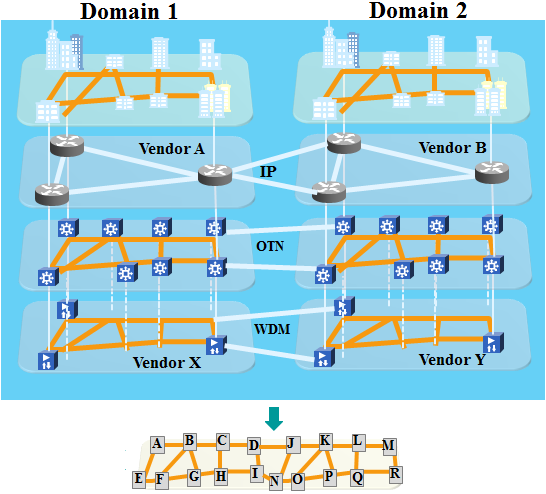
\includegraphics[scale=0.50]{MultiDomainLayer.png}
	\caption{Multi-Domain, Multi-Layer}
	\label{fig:MDL}
	\end{figure}
	
	Applications at the edges of these networks require datapath for exchange of data. For example, data
	center interconnects. Large amounts of data need to be exchanged between data centers. These data center
	applications require connectivity and bandwidth irrespective of the technology that is used to enable
	them. The underlying transport infrastructure could be IP, Packet/MPLS or Optical. If the resources viz.
	ports, links and bandwidth can be virualized with generic abstractions, all the applications would need
	is to program this \emph{\bf virtual overlay network} of devices interconnected by links (Fig.
	\ref{fig:MDL}). The network truly becomes open, programmable and flexible. \\
		
	\begin{figure}[htb]
	\centering
	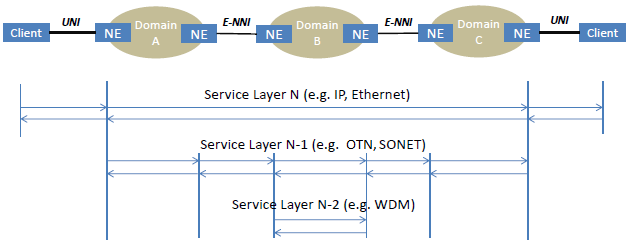
\includegraphics[scale=0.50]{MLwoOF.png}
	\caption{Service Provider Transport Network}
	\label{fig:MLwoOF}
	\end{figure}

	\textit{Open Transport Switch (OTS)} is an OpenFlow \cite{OF1.0} enabled light weight, virtual switch
	that manages a transport network element (NE). With a controller, the transport domain now could be
	controlled via SDN. Applications can now talk to the controller to request provision trunks of required
	capacity with additional QoS parameters if any. This gives service providers a unified view and of the
	network (Fig. \ref{fig:MLwOF}). This also greatly simplifies the control plane to manage NEs at multiple
	layers. The SDN Controller can interface with smart applications to perform path computation,
	provisioning and monitoring. The application requesting the bandwidth will only be concerned about the
	capacity and QoS guarantees. It is up to the controller (or the application talking to the controller) to
	find an end-to-end path going over multiple domains/layers, meeting the SLA.

	\begin{figure}[htb]
	\centering
	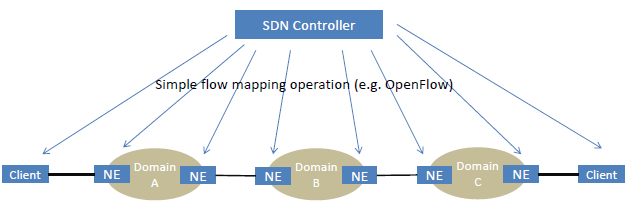
\includegraphics[scale=0.50]{MLwOF.png}
	\caption{SDN Enabled Transport Network}
	\label{fig:MLwOF}
	\end{figure}

	Fig. \ref{fig:OTSArch} shows the building blocks of OTS. Assuming the Controller can be reached at a well
	known location, the OTS agent can advertise the port, link and other reource information to the
	Controller as part of the handshaking. The \textit{Discovery Agent} is responsible for discovery and
	registration of SDN-controlled resources. It appropriately notifies the Controller dynamiclaly as and
	when NE state changes (for example, removal/addition of line or tributory modules). In OpenFlow, this
	typically happens via the switch \texttt{OFPT\_FEATURES\_REQUEST}, \texttt{OFPT\_FEATURES\_REPLY} and
	other related \texttt{Modify State} messages \cite{OF1.0}. How the discovery agent retrieves this
	information from the NE is upto the implementation or via proprietary vendor interfaces. \\
	
	The \textit{Control Agent} is responsible for monitoring and propagating notifications and alarms to the
	Controller. FCAPS is a very important component in transport networks. It lets the network admins monitor
	performance, faults and alarms in the network. Loss-of-light, Loss-of-sync, Loss-of-signal are some
	examples of alarms. Faults could range from link failures to equipment failures. (Note that some of
	equipment related alarms could be reported by both the Control and Discovery agents). This way, the
	controller's state is asynchronously (or synchronously) kept consistent with the state of the underlying
	network. The \textit{Dataplane Agent} is responsible to program the NE datapath to create/release
	circuits/LSP. The datapath entities could be Time slots, Cross connects (XCON) or MPLS labels. This
	programs the underlying network infrastructure and helps complete the datapath. The controller sends
	appropriate OpenFlow messages (similar to \texttt{OFPT\_FLOW\_MOD} message). Again, how the Dataplane
	Agent programs the particular NE database/forwarding tables could be through vendor specific interfaces. \\
	
	The northbound interface from OTS to the Controller is OpenFlow 1.0.0 \cite{OF1.0}. Given that OTS is
	virtualizing transport NE, much of the Ethernet centric OpenFlow messages are not used. With addition of
	extensions (see sections \ref{sec:ofext} \& \ref{sec:design}), the Controller can send requests to OTS
	to provision/release transport circuits.
	
	OTS being a virtual switch has multiple advantages associated:

	\begin{itemize}
	    \item OTS is stateless or very minimally stateful: All the alarms, stat counters, forwarding table entries are 
		stored in the NE database and could be retrieved by OTS. OTS need not maintain these managed objects. 
		This also allows for OTS to be light on resources.
	    \item OTS is lightweight and portable: Given that most of the state is maintained by the NE, if the southbound 
		interface from the OTS agent to the NE is flexible enough (implementation and vendor specific), the OTS 
		agent could be made to run on a standalone server or EMS or any other machine which can communicate 
		and maintain an active OpenFlow session with the Controller.
	    \item OTS Southbound Interface: The southbound interface from the OTS agent to the NE could also be 
		standard interfaces which allows OTS implementations to be multi-vendor ready. For example, TL-1 \cite{tl1} 
		is a widely used network element management protocol amongst RBOCs. If TL-1 is used to communicate between 
		OTS and the NE, we could potentially map OTS to any vendor's NE which can understand TL-1. Other
		examples include NETCONF \cite{netconf}
  	    \item Multiple OTS agents could be run on the same NE. These different instances can be given a restricted 
		view of the ports/wavelengths present on the NE and manage their respective resourcess only 
		(See section \ref{sec:otvs})
	\end{itemize}

	\begin{figure}[htb]
	\centering
	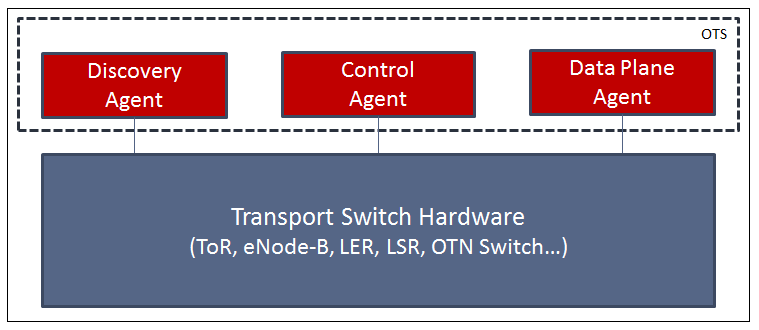
\includegraphics[scale=0.37]{OTSArch.png}
	\caption{OTS Building Blocks}
	\label{fig:OTSArch}
	\end{figure}

	\subsection{OpenFlow Extensions}
	\label{sec:ofext}
	
	OpenFlow \cite{OF1.0} is very L2/L3 centric as of today. Given that we want to control optical transport
	equipments, the protcol currently has no understanding of circuit switching constructs like time-slots or
	cross-connects (XCON). We are proposing extensions to OpenFlow by adding messages that allow provisioning/release of
	circuits. Given that we are virtualizing the network, we use opaque, MPLS-style labels to represent links
	(sequence of ingress/egress ports). We also indicate the style of circuit that needs to be setup (see
	section \ref{sec:modes}). Along with these, the message includes service rate and latency paramters along
	with provisioning actions (\texttt{ADD\_XCON} and \texttt{REM\_XCON}). For now, we assume the type of service/traffic 
	to be GbE. However, this could be OC-3, OTU3, Fiber Channel and so on.

	\begin{lstlisting}
struct ofp_id {
	// Host ID - DCN IP Address of the Node
	uint32_t node;

	// Flow ID maintained by the Controllre
	uint32_t label;
};

struct ofp_xconn {
	struct ofp_header header; // OFPT_VENDOR
	uint32_t vendor;  // Vendor ID

	uint8_t pad[4];
		  
	struct ofp_id src; // Source of the flow
	struct ofp_id dst; // Destination of the flow
		   
	uint32_t rate;     // Rate of service (Mbps)
	uint8_t latency; // Latency - 0 to 255
	uint8_t style;     // Implicit = 1 Explicit = 2

	// Unidirection = 1 Bidirectional = 2
	uint8_t directional;

	uint8_t pad_extra[1];

	// ADD_XCONN = 0xFF REM_XCONN = 0xFE
	struct ofp_action_header actions[0];
};
OFP_ASSERT(sizeof(struct ofp_xconn) == 40);
	\end{lstlisting}
	
	\subsection{Modes of Operation} \label{sec:modes}
	We already described how OTS architecture can simplify control plane by eliminating all the complex
	UNI/E-NNI/GMPLS routing and signaling protocols. Integrating OTS into today's large service provider transport
	networks may become a very complex exercise (we are infact trying to make transport networks more
	flexible and manageable!). Taking this into account, we propose two modes of operation to allow smooth
	integration of, and transition to trasnport SDN.

	\begin{figure}[htb]
	\centering
	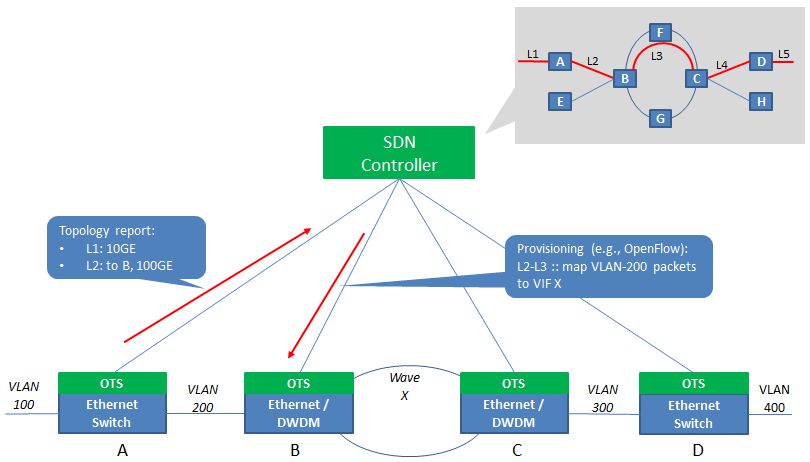
\includegraphics[scale=0.37]{OTSExplicit.png}
	\caption{Transport SDN Explicit Mode}
	\label{fig:OTSExplicit}
	\end{figure}

	\subsubsection{Explicit Mode}
	Fig. \ref{fig:OTSExplicit} depicts \textit{Explicit Mode}. In this mode, the Controller has the knowledge
	of every NE in every domain/layer. After optimal path computation, provisioning a circuit becomes a
	simple exercise of the Controller programming all the transport devices along the path in a hop-by-hop
	manner across single or multiple transport domains.
	
	\subsubsection{Implicit Mode} Fig. \ref{fig:OTSImplicit} depicts \textit{Implicit Mode}. In this mode,
	the Controller is aware of only the edge nodes in every transport domain (Ethernet/MPLS/OTN). Within the
	domain, the existing routing and signaling control plane can be used to setup intra-domain path. The
	Controller would send provisioning request, specifying the source and destination to the SDN-aware nodes
	at the edges of the network. The source node will then trigger MPLS/GMPLS control plane to setup the circuit.
	Controller being aware of NE type and capabilities, \textit{stitches} these segments across multiple
	domains to form an end-to-end circuit. Implicit mode adds great flexibility in gradually incorporating
	OTS architecture into existing transport networks. Without disrupting current deployments, service
	providers may choose to continue using intra-domain control plane while still being SDN aware. From a
	Controller's perspective, this edge-to-edge intra-domain path appears as a single network fabric of a
	given capacity. Service providers guagingt the necessary network management effort, can gradually make
	all the NEs SDN capable, moving to an explicit deployment model.

	\begin{figure}[htb]
	\centering
	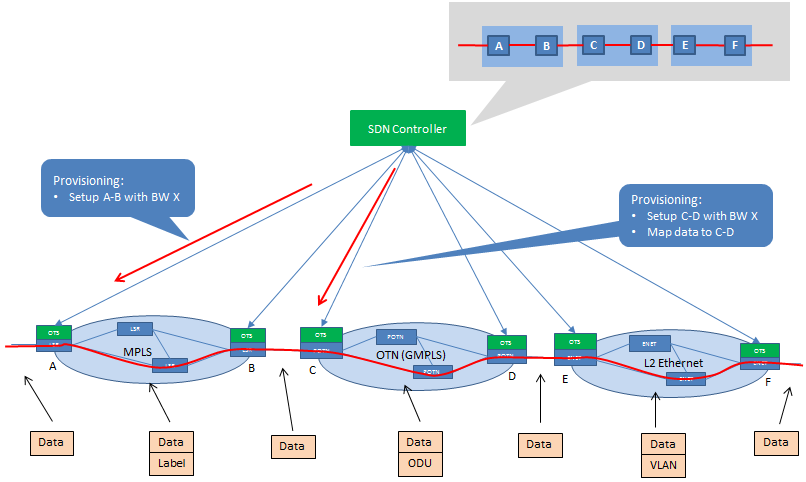
\includegraphics[scale=0.37]{OTSImplicit.png}
	\caption{Transport SDN Implicit Mode}
	\label{fig:OTSImplicit}
	\end{figure}

\section{Desgin and Implementation}
\label{sec:design}
	Section \ref{sec:arch} described the building blocks of OTS. The prototype OTS implementation only has the 
	Dataplane agent functionality built in. Rest of the subsystems will be integrated in the future. 

	\subsection{Controller}
	\label{sec:oscars}
	On-Demand Secure Circuits and Advanced Reservation System (OSCARS) \cite{oscars} is a provisioning system
	developed by Energy Sciences Network (ESnet). It provides multi-domain, high-bandwidth, virtual circuits
	that guarantee end-to-end network data transfer performance. OSCARS virtual circuits carry fifty percent
	of ESnet's annual 60 petabytes of traffic. (Fill in more details here) \\
	
	OSCARS has all the necessary components to provision and release circuits, and the path computation.
	OSCARS was extended by adding OpenFlow interfaces (including the extensions defined in section
	\ref{sec:ofext}). This makes OSCARS the SDN controller. OSCARS then establishes an OpenFlow session with
	OTS agent and sends appropriate messages to create/release transport circuits. The initial handshaking
	between OSCARS and OTS is as described in \cite{OF1.0}. Handshaking involves exchange of
	\texttt{OFPT\_HELLO}, \texttt{OFPT\_FEATURES\_REQUEST} and \texttt{OFPT\_FEATURES\_REPLY} messages.
	However, since many of the attributes in the messages are Ethernet centric, we hand fill them to values
	of our choice. We have retained the standard handshaking as per the spec to allow ease of adding
	transport extensions to other Controller implementations. The Controller sends OpenFlow extension
	messages to OTS for circuit provisioning/release.
	
	\subsection{OTS Agent - Virtual Switch}
	\label{sec:otvs}
	Our prototype OTS agent is bound to underlying physical transport NEs. Infinera DTN \cite{dtn} was used
	as the optical transport NE. DTN has fully flexible SONET/SDH, OTN and Ethernet add/drop
	capabilities with OTN \cite{otn} line side wavelength Optical Carrier Groups (OCG). It includes an
	embedded GMPLS control plane for end-to-end routing and provisioning. As part of the management suite,
	the DTN provides TL-1 interface to access the NE for troubleshooting, alarms and event
	notifications, equipment, fault and performance monitoring. The northbound OpenFlow interface (with
	transport extensions) was explained in the previous sections. We use TL-1 to interface OTS with the NE.
	For example, on receiving a circuit provisioning request from the Controller via OpenFlow, we convert
	that request to a TL-1 equivalent command and inject it into the NE. \\

	As for the tributory ports and the wavelengths to be used, we maintain a simple configuration file which
	is manually edited before OTS is started. Given that these are TDM circuits, incoming traffic payload is
	digitally wrapped/containerized into OTN optical channels and transported. There is no header or label
	lookup to be performed on incoming traffic. Hence we don't need to maintain any flow tables and this
	configuration file itself acts as a simple flow table\footnote{Note that if OTS needs to manage packet
	switching (PSN) core transport switches like MPLS switches, we would need a more detailed flowtable-like
	structure}. Due to virtualization, multiple OTS agents can be managing a subset of tributory ports/line
	side wavelenths on the same NE. Depending on the configuration file, we can make the OTS agent aware of
	only the specified ports and opitcal channels/OCGs. This adds various flexibilities. Service providers
	can sell wholesale bandwidth to multiple third party/tier-2 providers who will only be able to control a
	portion of the equipment which they have paid for. Another scenario could be two OTS agents, one active
	and another stand-by. If the active OTS instance goes down, the stand-by could take over.\\

	TL-1 is the southbound interface from OTS to the NE. The OTS agent establishes a TCP session with
	the TL-1 agent running on the NE. Once successful, OTS can now execute TL-1 commands over this
	channel (just like a network admin would). Using TL-1 gives the flexibility of running OTS instance
	outside the NE. We can run the OTS agent on a standalone server and establish a TL-1 session over
	TCP/IP with the TL-1 agent. Also, if OTS needs to manage NE of another vendor, given that TL-1 is a
	standardized interface, the migration should work without any hassles. Howver, there could be vendor 
	specific TL-1 commands which would have to be handled appropriately if necessary.

\section{Results and Observations}
\label{sec:results}
	\subsection{Testbed}
	\label{sec:testbed}
	We made use of ESnet's Long Island Metropolitan Area Network (LIMAN) to demonstrate SDN controlling the
	 transport optical backbone through OSCARS and OTS. Fig. \ref{fig:LIMAN} shows the testbed setup. DTN
	nodes A and B are SDN aware and two OTS agents were managing each of these NEs. The nodes connected
	to ESnet's production network via DWDM fibers. There also exists a direct fiber connectivity between the two
	nodes. There are two hosts with 40G Ethernet interfaces connected to each of these nodes. We setup two 40G 
	circuits between node A and B, one over the direct (one-hop) fiber link and another over the production node.
	The fiber path traversed by the circuit is transparent to the end hosts. The end hosts will see a direct one-hop
	IP Link connecting each other.

	\begin{figure}[htb]
	\centering
	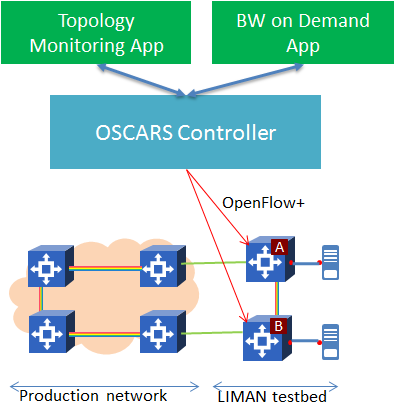
\includegraphics[scale=0.50]{LIMAN.png}
	\caption{Testbed Setup}
	\label{fig:LIMAN}
	\end{figure}

	\subsection{Measurements}
	\label{sec:measure}
	The measurements done were to reserve a 40G circuit from Node A to B (Fig. \ref{fig:LIMAN}). This only includes the time 
	taken by the Controller to compute the path and to send the ofp\_xconn message. This doesn't include the variable
	network time for the message to reach OTS and for the optical transport NE XCON programming and/or GMPLS control
	messaging. These are not significant from the point of view of transport networks/NE as these are vendor/equipment
	specific (XCON programming) and much of the latency in GMPLS messaging is due to fiber propogation delay. The control
	plane messaging and NE timeslot programming is also dependent on the topology.

	\begin{center}
		\begin{tabular} { |  c | c | c | c | }
			\hline
			 Min & Max & Mean & Std. Dev \\ \hline
			2	 & 7 & 2.84 & 0.98 \\
			\hline
		\end{tabular}
		\captionof{table}{Circuit path computation latencies (s)}
		\label{tab:measurements}
	\end{center}

	Given a fairly simple topology, the maximum latency observed is for the first circuit setup request. OpenFlow session needs
	to be established with the OTS agents and hence the higher latency. Once the session is active, the time involved is for the
	Controller to compute path based on the knowledge it has about the topology. Since this is a protoype, most of the topology
	and node/link information is statically configured. The OTS Discovery agent is responsible to provide the Controller with the
	necessary topology and network resource information.

\section{Scope for Future Work}
\label{sec:future}
	There are several additions to OTS that could provide full network virtualization capabiliites. From an
	implementation perspective, we wish to fully integrate the Monitoring and the Discovery agents into
	OTS for fault/alarm propogation and port/link discovery respectively. Currently, the ports, optical 
	channels and links are hand-configured through a configuration file for this prototype implementation.
	But we would need a dedicated info model similar to Open vSwitch Database \cite{ovsdb} to store
	these configuration information and advertise it to the Controller. This allows the Controller to discover
	the complete topology depending on the mode of operation (Implicit/Explicit). JSON formatted data 
	could be used to exchange these topology extracts between OTS and the Controller. Security is another
	key aspect in the system. Our implementaiton uses long-lived TCP/IP sessions between the Controller
	and the OTS agent. SSL/TLS sessions could be used instead. \\

	From the point of view of standardization, many important functions that are inherent to core transport networks
	have to be factored in. For example, protection and restoration. Typically, most of these today are part of the
	control plane (MPLS FRR or GMPLS restoration).Thorough investigations need to happen if
	these have to be incorporated into OpenFlow. Or, these could continue to be a part of the underlying control
	plan as in the case of Implicit mode. Further, if domain specific parameters (like optical impairments, OSNR etc)
	are needed, these need not be a part of the protocol itself. Instead, a management interface like OFConfig or
	NetConf can be used to extract these.

\section{Conclusion}
	We have demostrated a prototype virtual transport switch for optical long haul networks. OTS can be
	estended to a packet switched IP/MPLS (PSN) core backbone too. The idea of extending Software Defined
	Networking concepts to transport provides compelling technical and economical advantages to large service
	providers to efficiently engineer, manage and evolve their networks. Network virtualization through OTS
	allows building an overlay network that applications can program to meet their specific bandwidth
	requirements irrespective of what underlying layers (L1/L2/L3) or technologies (OTN/MPLS/IP) are used.
	With addition of appropriate extensions to OpenFlow, the transport infrastructure can be made more open
	and programmable which allows multi-laye, multi-domain and multi-vendor optimizations in both core and
	metro networks. Efforts are already underway within Open Networking Foundation (ONF) to allow
	standardization of transport extensions to OpenFlow (NewTransport WG). We hope HotSDN acts as
	a catalyst and provides a forum for the discussion of these ideas.

\bibliographystyle{acm}
\bibliography{ots} 

\end{document}